\documentclass{llncs}

\usepackage{epsfig}
\usepackage{graphicx}
\usepackage{hyperref}
\usepackage{url}
\usepackage{cleveref}
\usepackage{hhline}
\usepackage{subcaption}

\begin{document}

%----------------------------------------------------------------------
       
\title{Using Metric Space Indexing for Complete and Efficient Record Linkage}

%----------------------------------------------------------------------

\author{{\"O}zg{\"u}r Akg{\"u}n\inst{1} \and Alan Dearle\inst{1}
  \and Graham Kirby\inst{1} \and Peter Christen\inst{2}}

\institute{School of Computer Science, University of St Andrews,
St Andrews, Scotland. Contact: \email{\{ozgur.akgun, alan.dearle, graham.kirby\}@st-andrews.ac.uk}
\and
Research School of Computer Science, The Australian National University,\\
Canberra, Australia. Contact: \email{peter.christen@anu.edu.au}}
      
%----------------------------------------------------------------------

\maketitle

\begin{abstract}

Record linkage is the process of identifying records that refer to the
same real-world entities in situations where entity identifiers are
unavailable. Records are linked on the basis of similarity between
common attributes, with every pair being classified as a link or
non-link depending on their similarity. Linkage is usually performed in
a three-step process: first, groups of similar candidate records are
identified using indexing, then pairs within the same group are compared
in more detail, and finally classified. Even state-of-the-art indexing
techniques, such as locality sensitive hashing, have potential
drawbacks. They may fail to group together some true matching records
with high similarity, or they may group records with low similarity,
leading to high computational overhead. We propose using \emph{metric
space indexing} (MSI) to perform \emph{complete} linkage, resulting in a
parameter-free process combining indexing, comparison and classification
into a single step delivering complete and efficient record linkage. An
evaluation on real-world data from several domains shows that linkage
using MSI can yield better quality than current indexing techniques,
with similar execution cost, without the need for domain knowledge or
trial and error to configure the process.

\end{abstract}

\keywords Entity resolution; data matching; similarity search;
         blocking.

%----------------------------------------------------------------------

\section{Introduction}
\label{sec-intro}

Record linkage, also known as entity resolution, data matching and
duplicate detection~\cite{Chr12}, is the process of identifying and
matching records that refer to the same real-world entities within or
across datasets. The entities to be linked are often people (such as
patients in hospital or customers in business datasets), but record
linkage can also be applied to link consumer products or bibliographic
records~\cite{Chr12}. Record linkage is commonly challenged by the lack
of unique entity identifiers (keys) in the datasets to be linked, which
prevents the use of a database join. Instead, the linkage of records
requires the comparison of the common attributes (or fields) that are
available within the datasets, for example the names, addresses and
dates of birth of individuals.

To overcome data quality issues such as typographical errors and
variations (common in name and address values~\cite{Chr12}), approximate
string comparison functions (e.g. edit distance, the Jaro-Winkler
comparator, or Jaccard similarity~\cite{Chr12}) are used to compare
record pairs, leading to a vector of similarities (one similarity per
attribute compared) for each pair. These are used to classify the record
pairs into \emph{links} (where it is assumed both records correspond to
the same real-world entity) and \emph{non-links} (where they are assumed
to correspond to different entities). Various classification methods
have been employed in record linkage~\cite{Chr12,Don15}, ranging from
simple threshold-based to sophisticated clustering, supervised
classification, and active learning approaches~\cite{Wan15}.

Besides a lack of unique entity identifiers, and data quality issues,
linkage is also challenged by dataset scale~\cite{Don15}. To avoid full
pair-wise comparison of all possible record pairs (quadratic in the
dataset sizes), blocking techniques, commonly known as
\emph{indexing}~\cite{Chr12b}, are used. These split the datasets into
smaller blocks in an efficient way, grouping together records that are
likely to correspond to the same entity. Only records within blocks are
then compared in detail.

While indexing allows efficient linkage of large datasets~\cite{Don15},
scalability is at the cost of reduced linkage quality, because
potentially matching record pairs are ignored, leading to lower
recall~\cite{Chr12}. Indexing techniques, discussed in more detail
later, range from simple phonetic based blocking~\cite{Chr12} and
sorting of the datasets~\cite{Dra12} to locality sensitive hashing based
techniques~\cite{Kim10,Steorts2014}, and unsupervised~\cite{Kej13,Ram15}
and supervised~\cite{Bil06,Mic06} learning of optimal blocking schemes.


%----------------------------------------------------------------------

\begin{figure}[!t]
  \centering
  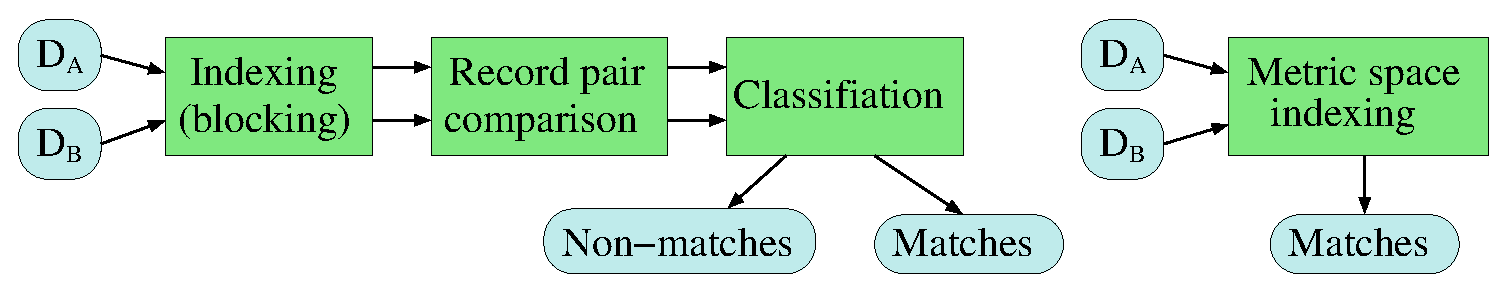
\includegraphics[width=1.0\textwidth]{figures/linkage-process}
  \caption{Overview of the steps of the traditional record linkage
           process (left side) and our proposed metric space
           indexing based approach (right side), as described in
           Sect.~\ref{sec-intro}, where records from two datasets,
           $\mathbf{D}_A$ and $\mathbf{D}_B$, are being linked.}
           \label{fig-rl-process}
\end{figure}

%----------------------------------------------------------------------

Traditional linkage systems that perform indexing prior to comparison
and classification (on the left in Fig.~\ref{fig-rl-process}) add a
further complexity. Indexing, comparison and classification are often
conducted using algorithms and parameters selected using domain
expertise, followed by manual assessment of the linkage
outcomes~\cite{Chr12}. If the resulting link quality is too low for a
certain application, the process is repeated with different parameter
settings or algorithms, giving a time-consuming iterative
process~\cite{Fis15}. The choice of an appropriate indexing technique
as well as suitable parameter settings (including which attributes to
use in indexing) will significantly affect the final linkage outcome.

We focus on approaches using a similarity threshold to classify links.
These are fundamentally limited by the extent to which true matching
records are similar, and true non-matches are dissimilar---this is
dataset-dependent. Within this domain, we define a technique to be
\emph{complete} if it guarantees to find all record pairs within the
specified threshold. Many indexing techniques are incomplete, since they
reduce computational cost at the expense of potentially overlooking some
true matches. By definition, incomplete techniques yield lower recall
than complete ones. Conversely, and counter-intuitively, complete
techniques can yield lower precision with some datasets. This is
discussed further in Sect.~\ref{sec-approach}.

Metric space indexing (MSI) is a complete technique with lower
computational cost than a brute force approach. It allows indexing,
comparison and classification to be combined into a single step (on the
right in Fig.~\ref{fig-rl-process}), making the process simpler, more
efficient and more effective than incomplete approaches.

The motivation for this work is the Digitising Scotland
project~\cite{Dibben2012}, which aims to transcribe and link all civil
registration events recorded in Scotland between 1856 and 1973. This
dataset will include around 14 million birth records, 11 million death
records and 4 million marriage records.

\smallskip
\textbf{Contribution:} Our primary contribution is the novel application
of MSI to achieve complete and efficient record linkage, without the
need for complex parameter tuning. We evaluate our approach on several
real-world datasets and demonstrate its advantages over existing
indexing techniques for record linkage.

\section{Related Work}
\label{sec-related}

We review relevant work in the areas of indexing for record linkage (for
recent surveys see~\cite{Chr12b,Pap16}), and metric space
indexing~\cite{Zezula2010}. Techniques to link records have been
investigated for over five decades~\cite{Fel69,New59}, with scalability
being an ongoing challenge as datasets grow in size and complexity.
Traditional blocking~\cite{Chr12b} uses a set of attributes (a
\emph{blocking key}) to insert records with the same value(s) in their
blocking key into the same block. Only records within the same block are
 compared to each other. To overcome variations and misspellings, the
values can be phonetically encoded using functions such as Soundex,
NYSIIS, or Double-Metaphone~\cite{Chr12}. These convert a string into a
code according to its pronunciation, assigning the same code to similar
sounding names (such as `Gail' and `Gayle'). Multiple blocking keys may
also be used to deal with missing attribute values.

A different approach uses sorted neighbourhoods~\cite{Mon96}, where the
datasets are sorted according to a \emph{sorting key} (usually a
concatenation of several attribute values). A sliding window is moved
over the datasets and only records within the window are compared.
Techniques that adaptively shrink or expand the window size based on the
characteristics of the sorting key values have been shown to improve
both linkage efficiency and quality~\cite{Dra12}.

These techniques are heuristics, requiring domain knowledge, such as the
choice of appropriate blocking or sorting keys. Poor choices of blocking
attributes result in records being inserted into inappropriate blocks,
and thus true matches being missed, giving \emph{incomplete} linkage.
Conversely, many pairs compared in a block may have low similarity,
being non-matches, giving \emph{inefficient} linkage.

Locality sensitive hashing (LSH), proposed for efficient
nearest-neighbour search in high-dimensional spaces~\cite{Ind98}, has
been used for record linkage indexing. Attribute values are hashed
multiple times, and blocks are created from those records that share
some hash values. \emph{HARRA}~\cite{Kim10} is a linkage approach based
on MinHash~\cite{Broder1997} and LSH which blocks, compares, and then
merges linked records iteratively. \cite{Steorts2014} evaluates two LSH
variations, concluding that to get good results, they must be tuned to
the datasets. This requires good ground truth data which may be
unavailable in real-world applications or expensive to obtain.

Metric space indexing (MSI) techniques~\cite{Zezula2010} support
similarity search. They require a distance measure between records, with
certain properties including the \emph{triangle
inequality}~\cite{Zezula2010}. Similarity search operations include
\emph{range-search(\textbf{q},d)}, identifying all records within a
distance $d$ of a query record $\mathbf{q}$;
\emph{nearest-neighbour(\textbf{q})}, returning the record with smallest
distance to $\mathbf{q}$; and \emph{nearest-n(\textbf{q},n)}, returning
the $n$ closest records to $\mathbf{q}$. Here we choose one MSI
structure, the M-tree~\cite{Ciaccia97indexingmetric}, and investigate
its efficacy for record linkage. The M-tree is dynamically balanced.
Every node contains a reference to a record being indexed, a pointer to
its parent, the distance to its parent, and the node's radius. The
radius of a node is the distance from it to its furthest child. For a
parent node with radius \textit{r}, all its children may be visualised
as being contained within a ball of radius \textit{r} from it.

A linkage method using R-trees~\cite{Hjaltason1998} was described
in~\cite{Li2006}, demonstrating that high linkage quality can be
achieved using Jaccard similarity. \cite{Ciaccia97indexingmetric} shows
that M-trees are almost always more efficient than R-trees, hence their
use here.

%----------------------------------------------------------------------

\section{Approach}
\label{sec-approach}

We address the following general linkage problem: for two datasets
$\mathbf{D}_A$ and $\mathbf{D}_B$, we wish to find, for each record in
$\mathbf{D}_A$, all the records in $\mathbf{D}_B$ that match it with
regard to a certain distance threshold $d$ (i.e.\ have a distance of $d$
or less). We compare several linkage algorithms: traditional blocking,
an incomplete similarity search method, LSH-MinHash, and a complete
method, M-tree. We also use a complete brute force technique as a
baseline, though this can only feasibly be applied to our smallest
dataset. All experiments have a number of parameters to configure the
search space and algorithm behaviour, including the distance function
and the threshold, $d$, specifying the maximum distance for two records
to be classified as a link (i.e.\ referring to the same entity). We
focus on a single distance function in these experiments, to constrain
the experimental space. In Sect.~\ref{sec-concl} we return to the
selection of alternative distance functions.

\textbf{Brute force:} Every record in $\mathbf{D}_A$ is compared with
every record in $\mathbf{D}_B$. Each pair is classified as a link if
the distance between the records is less than or equal to the
threshold $d$. This always finds all links, with complexity
$ O(|\mathbf{D}_A| \cdot |\mathbf{D}_B|)$.

\textbf{Traditional blocking:} The parameters are the set of blocking
keys and (optionally) the phonetic encodings applied to each attribute.
These are selected as described in~\cite{Chr12b}, exploiting knowledge
of the domain and of the data, and chosen with the intention of giving
the best possible results. Each record in $\mathbf{D}_A$ is placed into
the appropriate block based on its blocking key value. The algorithm
then iterates over the records in $\mathbf{D}_B$, and for each one
compares it with each of the records from $\mathbf{D}_A$ in the block
with the same blocking key value.

\textbf{LSH-MinHash:} The parameters for LSH-Minhash
are~\cite{Broder1997} \emph{shingle size} ($l_{ss}$), \emph{band size}
($l_{bs}$) and \emph{number of bands} ($l_{nb}$). First, the attributes
of each record in $\mathbf{D}_A$ are concatenated, and the result
\emph{shingled} into a set of n-grams with $n = l_{ss}$. Next, a set of
deterministically generated hash functions is applied to each n-gram in
the set and the smallest result (the MinHash) of each hash application
is added to a signature for the record. The number of hashes used, and
thus the size of the signature, is set to $l_{nb} \times l_{bs}$.
Finally, the signature is split into $l_{nb}$ bands and the values from
each band are hashed again to create a number of keys. The original
record is added to a map associated with each of the keys. To perform
linkage, the algorithm iterates over the records in $\mathbf{D}_B$. Each
record is hashed as described above, to obtain a set of keys. Each key
is looked up in the data structure, and the associated records from
$\mathbf{D}_A$ added to the result set. Finally, the record from
$\mathbf{D}_B$ is compared in turn with each record in the result set,
with the pair being classified as a link or non-link based on their
distance.

\begin{table}[t]
\caption{Characteristics of datasets used in the experiments.}
 \label{table-datasets}
  \centering
  \begin{scriptsize}
  \begin{tabular}{ccccc}
  \hline\noalign{\smallskip}
  Dataset~ & ~Records in~& ~Records in~ & ~Number of true~& ~Entities \\
    name(s)  & ~dataset $\mathbf{D}_A$~ & ~dataset $\mathbf{D}_B$~ &
    matching pairs & linked \\
  \noalign{\smallskip} \hline \noalign{\smallskip}
  Cora & 1,295 & 1,295 & 17,184 & Publication--Publication\\
  ~Isle of Skye~ & 17,612 & 12,284& 2,900 & Birth--Death \\
  Kilmarnock & ~38,430~ & ~23,714~ & ~8,300~ & ~Birth--Death~ \\
  \noalign{\smallskip} \hline
  \end{tabular}
  \end{scriptsize}
\end{table}

In some circumstances, incomplete approaches such as traditional
blocking and LSH-MinHash can yield higher precision than complete
techniques. This can occur when a significant number of non-matches
nonetheless have high similarity. In this situation, the fact that an
incomplete technique omits consideration of some potential links can
serve to improve precision, since a classification decision based on a
certain similarity threshold is incorrect for high-similarity
non-matches. By definition, recall can never be higher for incomplete
techniques.

\textbf{M-tree:} The linkage algorithm has no additional parameters. As
with \emph{LSH-MinHash}, each record in $\mathbf{D}_A$ is inserted into
an M-tree. To perform linkage, the algorithm iterates over each record
$\mathbf{b} \in \mathbf{D}_B$. A \emph{range-search(\textbf{b},d)}
operation is performed on the M-tree, passing the distance threshold $d$
as the second parameter. All the returned records are directly
classified as links.

%----------------------------------------------------------------------

\section{Experiments and Results}
\label{sec-exp}

We now describe the datasets and method used in our
evaluation~\footnote{The raw experimental data, additional figures and
the source code required to run these experiments can be downloaded
from the following repository. \\
\url{http://github.com/digitisingscotland/pakdd2018-metric-linkage}.}.
We used three datasets from two
domains in our experiments, as summarised in Table~\ref{table-datasets}.
The first is \emph{Cora}~\cite{Cora2017}, which contains 1,295 records
that refer to 112 machine learning publications. Cora is commonly used
as a benchmark dataset in the literature for assessing linkage
algorithms. Ground truth is provided via a unique \emph{paper\_id}
identifier of the form ``blum1993". In this experiment linkage is
performed over the same set of records (i.e.\ a
de-duplication~\cite{Chr12}).

The other two datasets are historical Scottish records of vital events
(birth, marriages and deaths), one registered on the \emph{Isle of
Skye}, a rural district, and the other records from \emph{Kilmarnock},
an industrial town. These datasets were created, curated and linked by
historical demographers~\cite{reid2006,reid2002}. Both include the names
and genders of individuals and their parents. Ground truth was generated
by the demographers based on their extensive domain knowledge.

In all of our experiments we use a single distance metric: the sum of
the attribute-level Levenshtein~\cite{Levenshtein66} edit distances.

% - - - - - - - - - - - - - - - - - - - - - - - - - - - - - - - - - - 

\subsection{Cora Results}

\begin{figure}
\centering
\begin{subfigure}{.47\textwidth}
  \centering
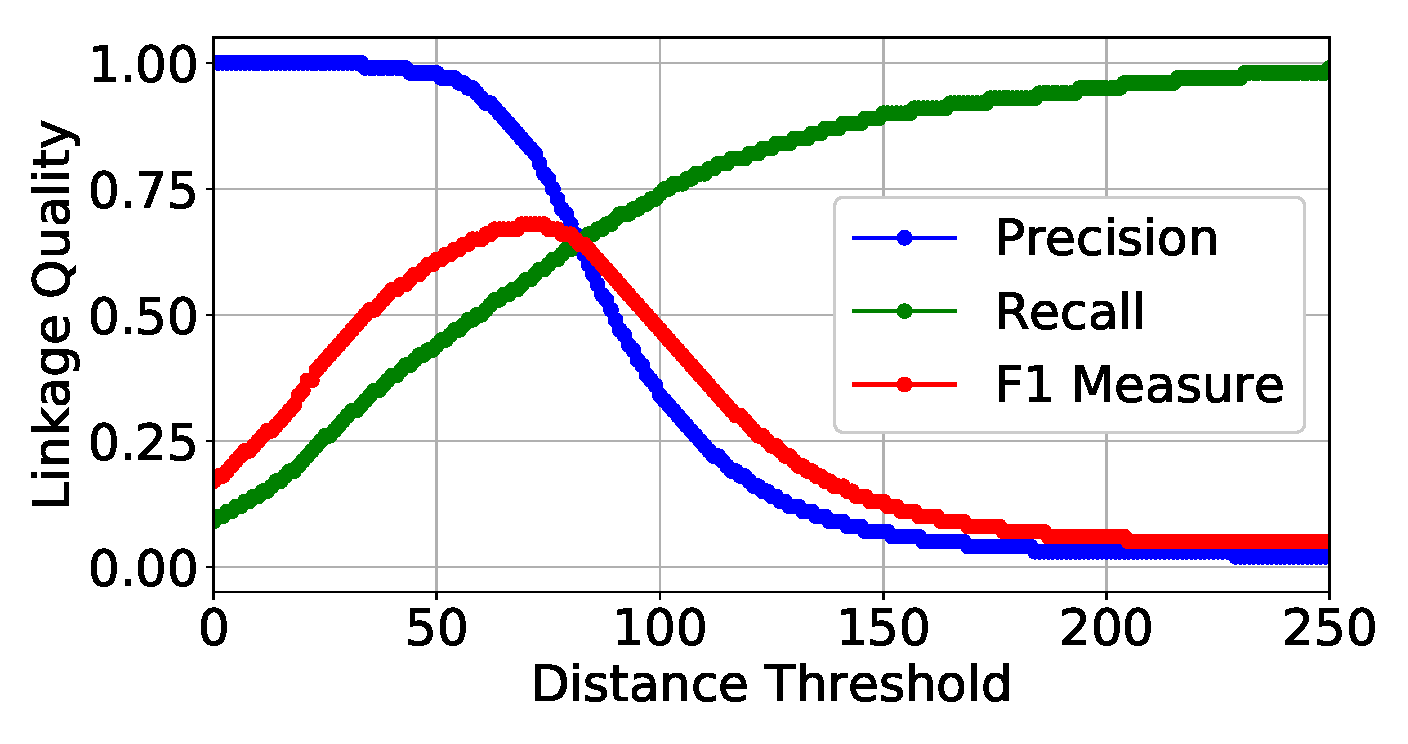
\includegraphics[width=\textwidth]{figures/plotLQ-cora-brute}
\vspace{-6mm}
\caption{Brute Force}
\end{subfigure}%
~~
\begin{subfigure}{.47\textwidth}
  \centering
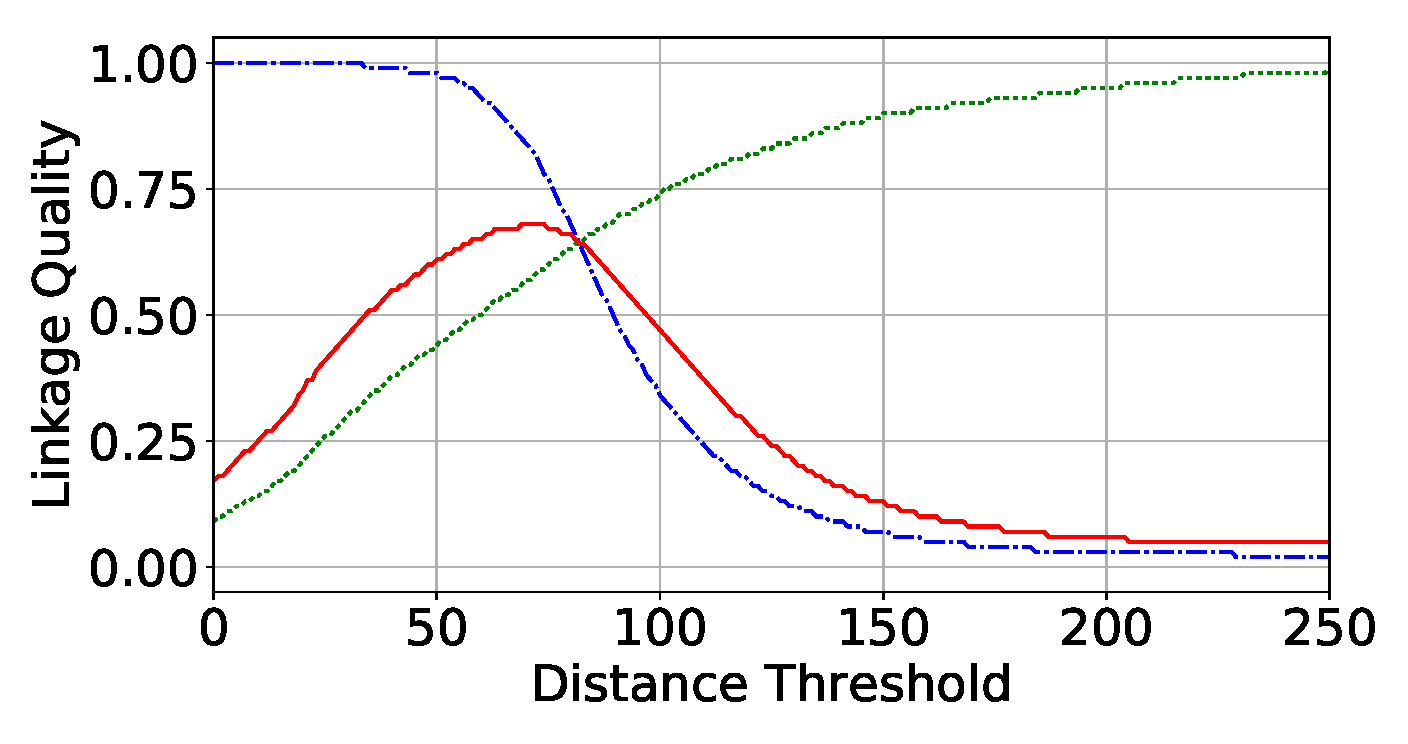
\includegraphics[width=\textwidth]{figures/plotLQ-cora-mtree}
\vspace{-6mm}
\caption{M-tree}
\end{subfigure} \vspace{3mm}

\begin{subfigure}{.47\textwidth}
  \centering
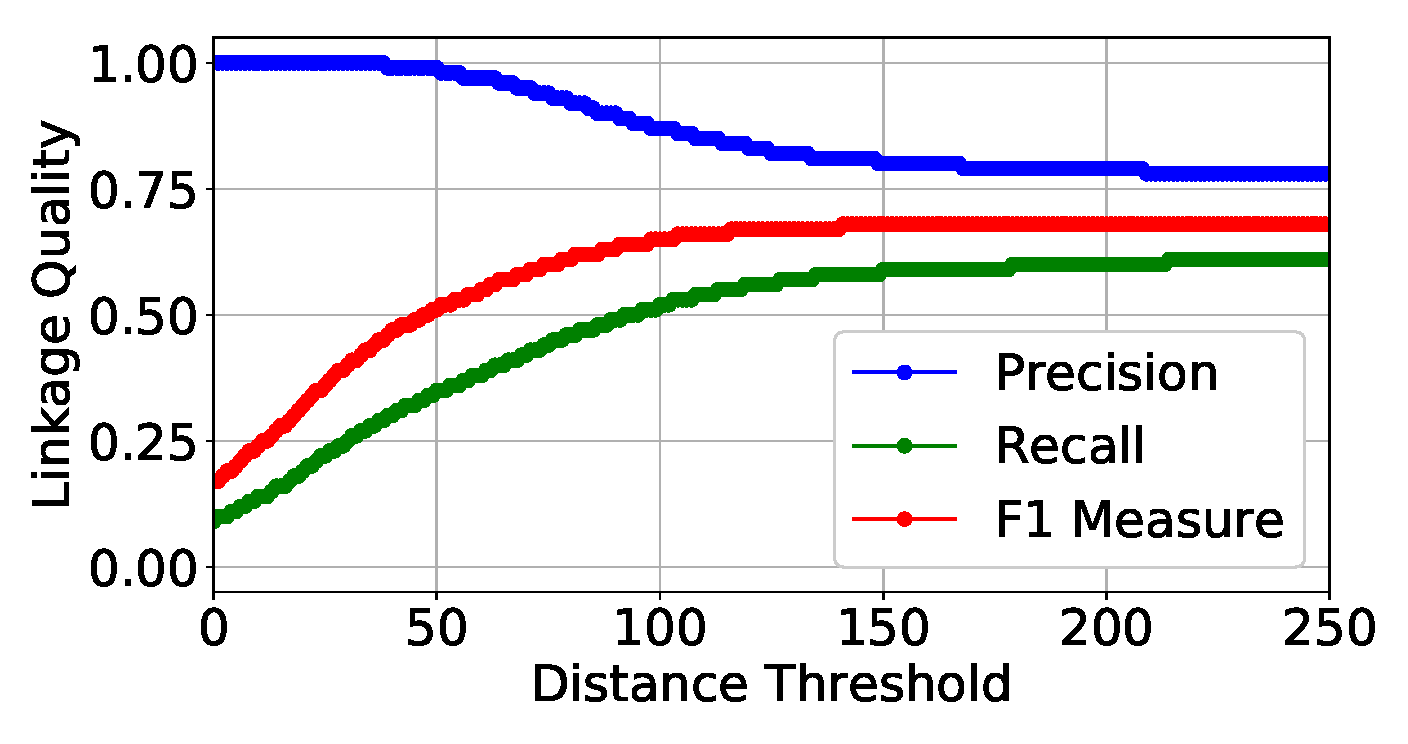
\includegraphics[width=\textwidth]{figures/plotLQ-cora-trad-authors}
\vspace{-6mm}
\caption{Blocking on `authors' attribute}
\end{subfigure}%
~~
\begin{subfigure}{.47\textwidth}
  \centering
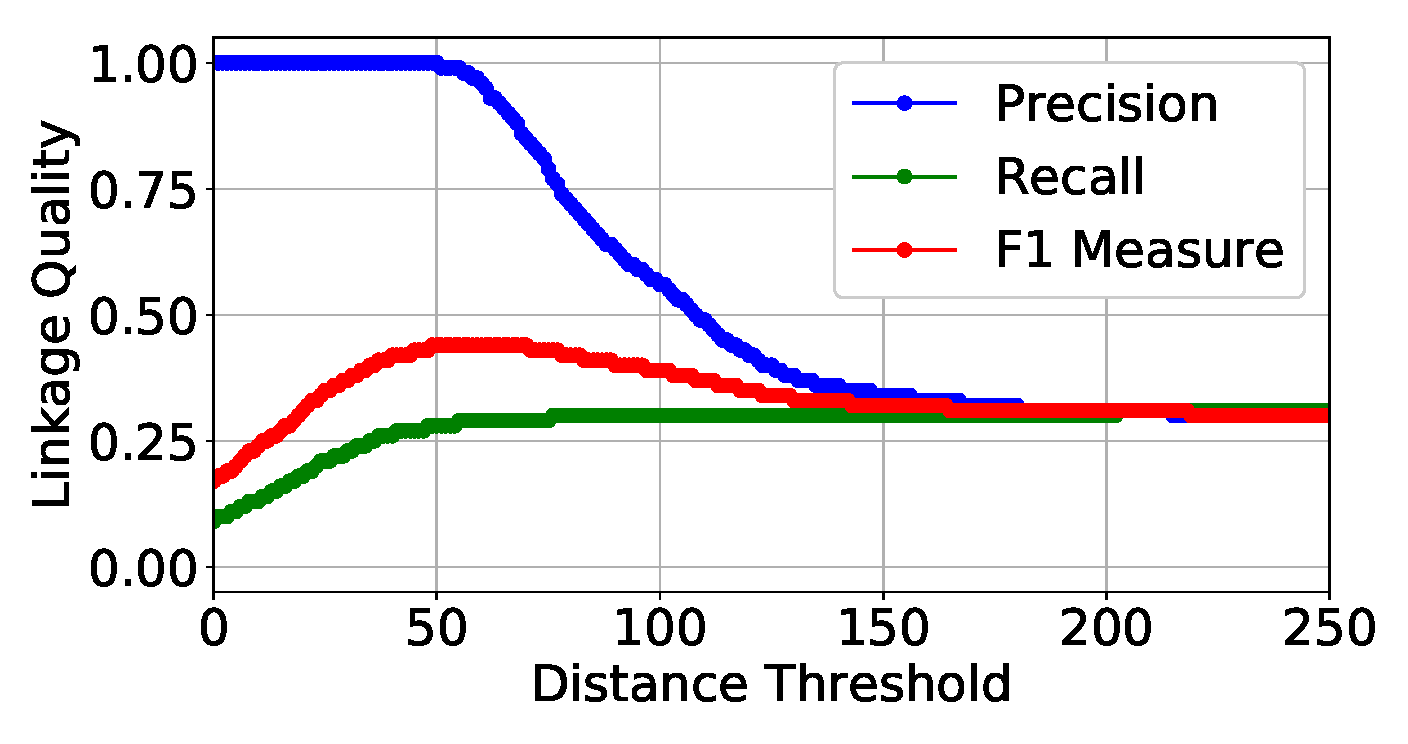
\includegraphics[width=\textwidth]{figures/plotLQ-cora-trad-title}
\vspace{-6mm}
\caption{Blocking on `title' attribute}
\end{subfigure} \vspace{3mm}

\begin{subfigure}{.47\textwidth}
  \centering
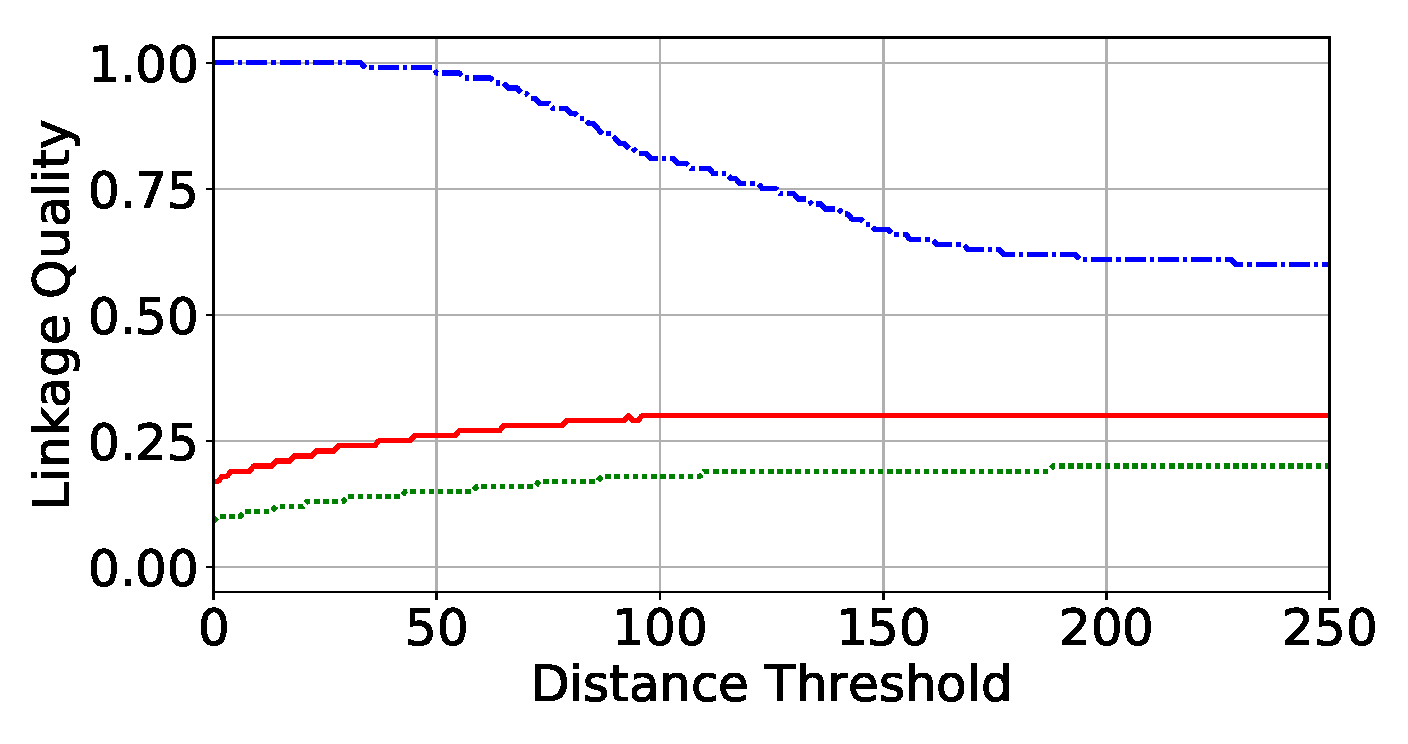
\includegraphics[width=\textwidth]{figures/plotLQ-cora-trad-year}
\vspace{-6mm}
\caption{Blocking on `publication year' attr.}
\end{subfigure}%
~~
\begin{subfigure}{.47\textwidth}
  \centering
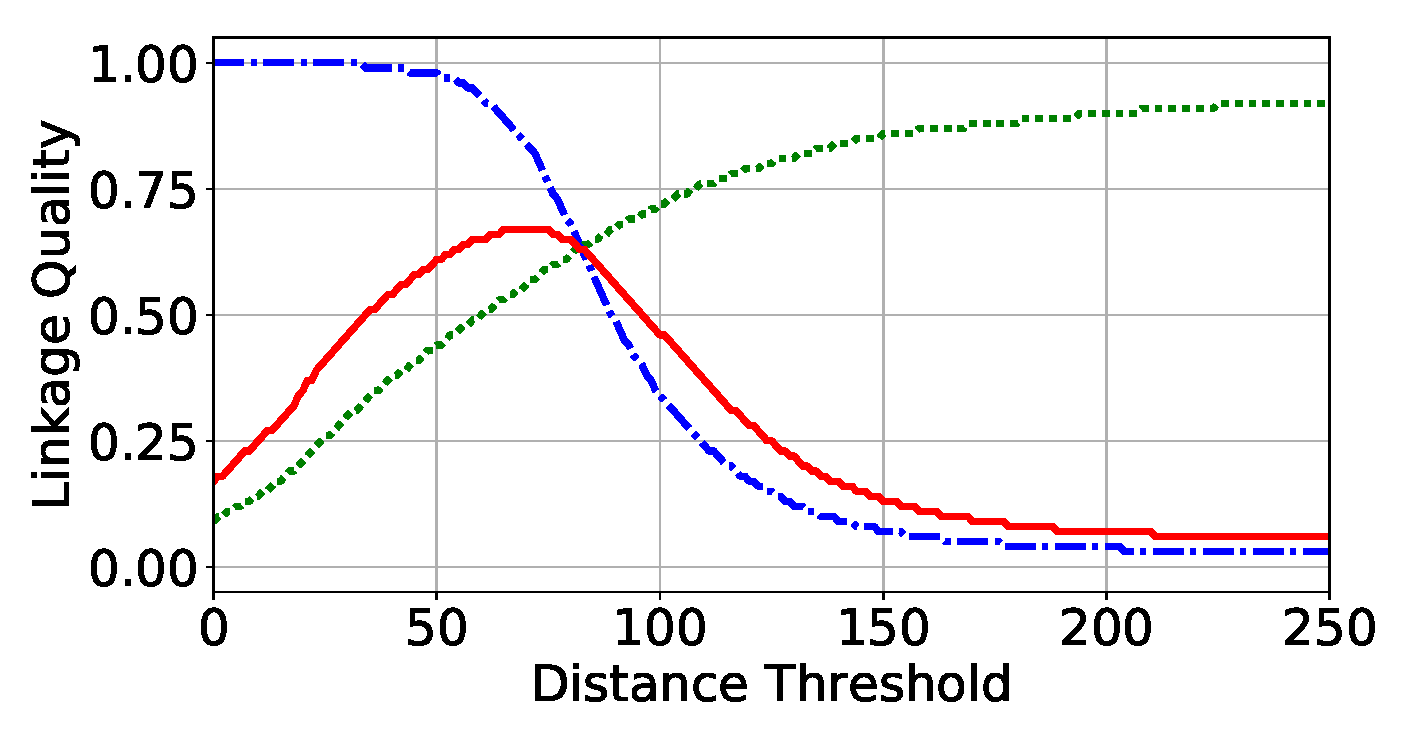
\includegraphics[width=\textwidth]{figures/plotLQ-cora-trad-combined}
\vspace{-6mm}
\caption{Blocking using the union of all attrs.}
\end{subfigure} \vspace{3mm}

\begin{subfigure}{.47\textwidth}
  \centering
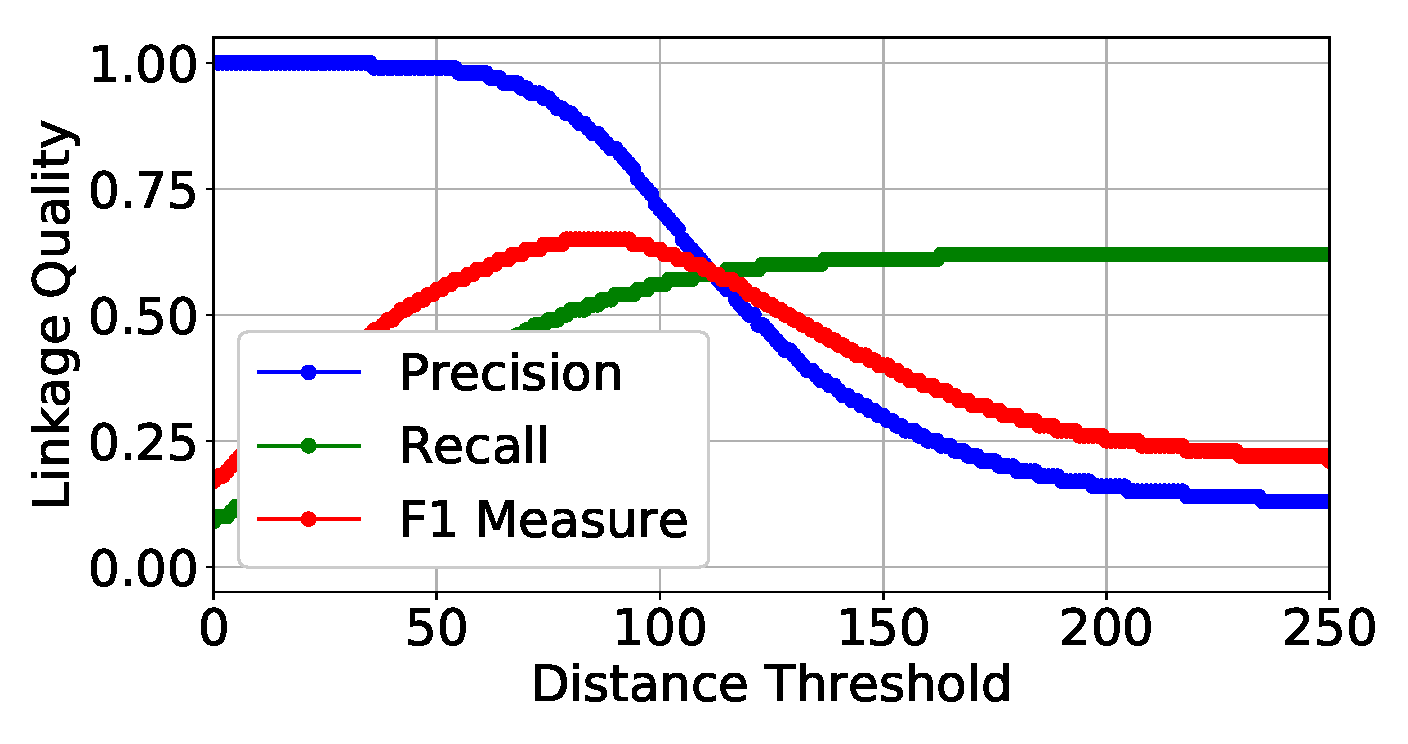
\includegraphics[width=\textwidth]{figures/plotLQ-cora-lsh-2-2}
\vspace{-6mm}
\caption{LSH using 2 bands of size 2}
\end{subfigure}%
~~
\begin{subfigure}{.47\textwidth}
  \centering
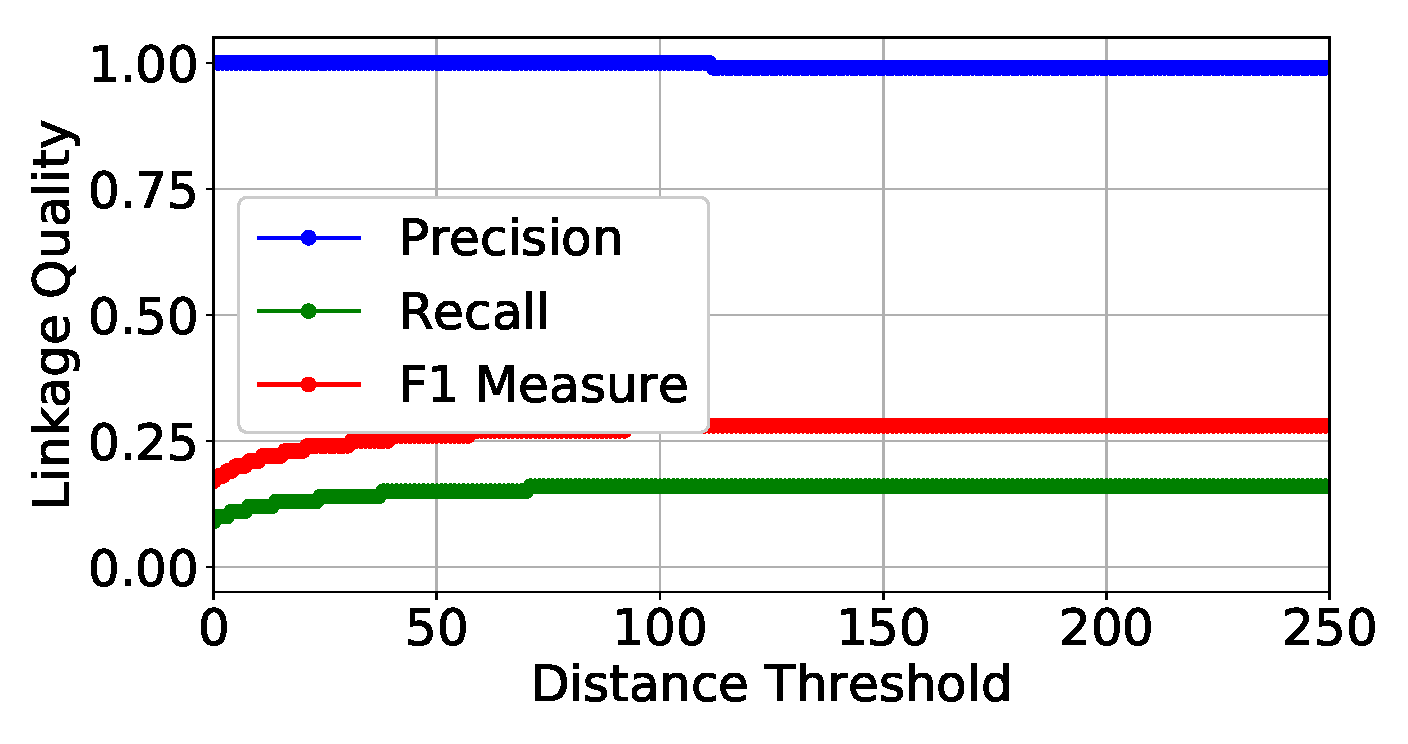
\includegraphics[width=\textwidth]{figures/plotLQ-cora-lsh-2-10}
\vspace{-6mm}
\caption{LSH using 2 bands of size 10}
\end{subfigure} \vspace{3mm}

\begin{subfigure}{.47\textwidth}
  \centering
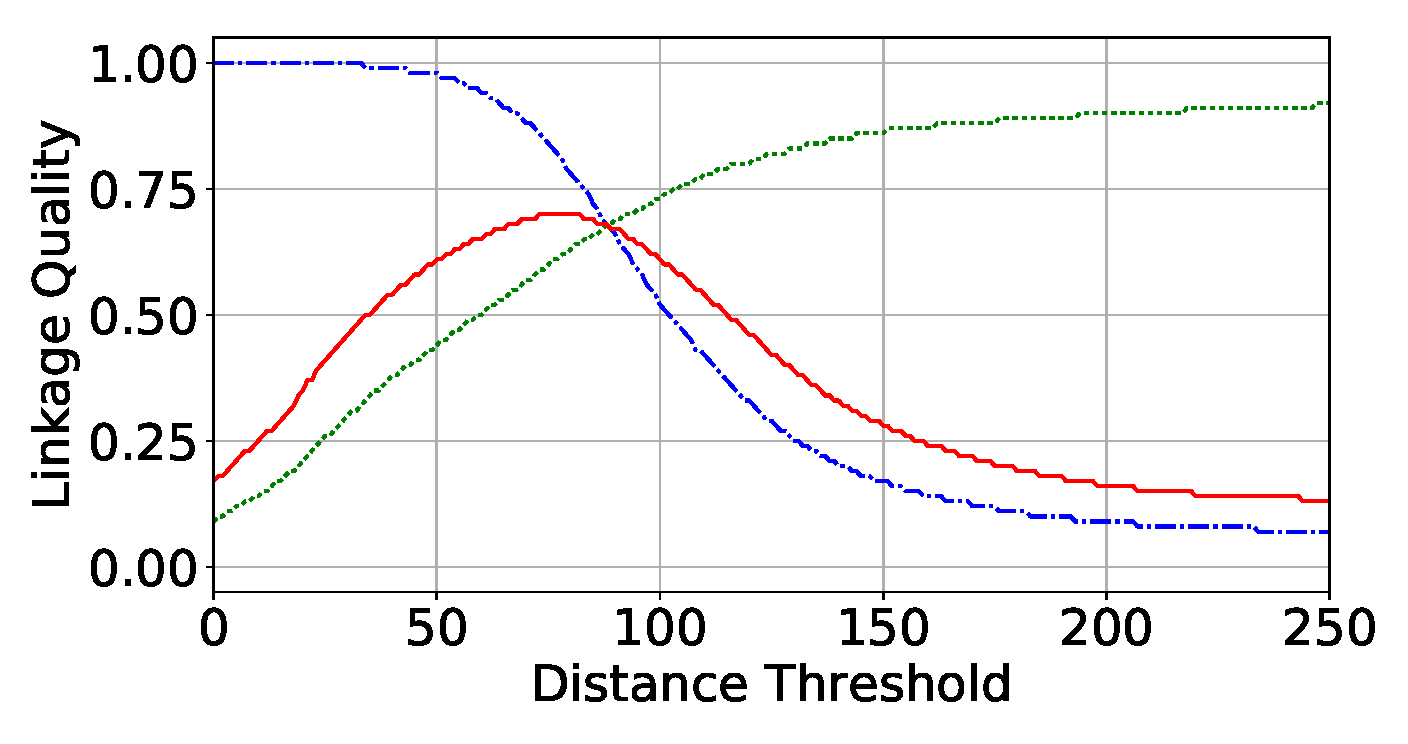
\includegraphics[width=\textwidth]{figures/plotLQ-cora-lsh-10-2}
\vspace{-6mm}
\caption{LSH using 10 bands of size 2}
\end{subfigure}%
~~
\begin{subfigure}{.47\textwidth}
  \centering
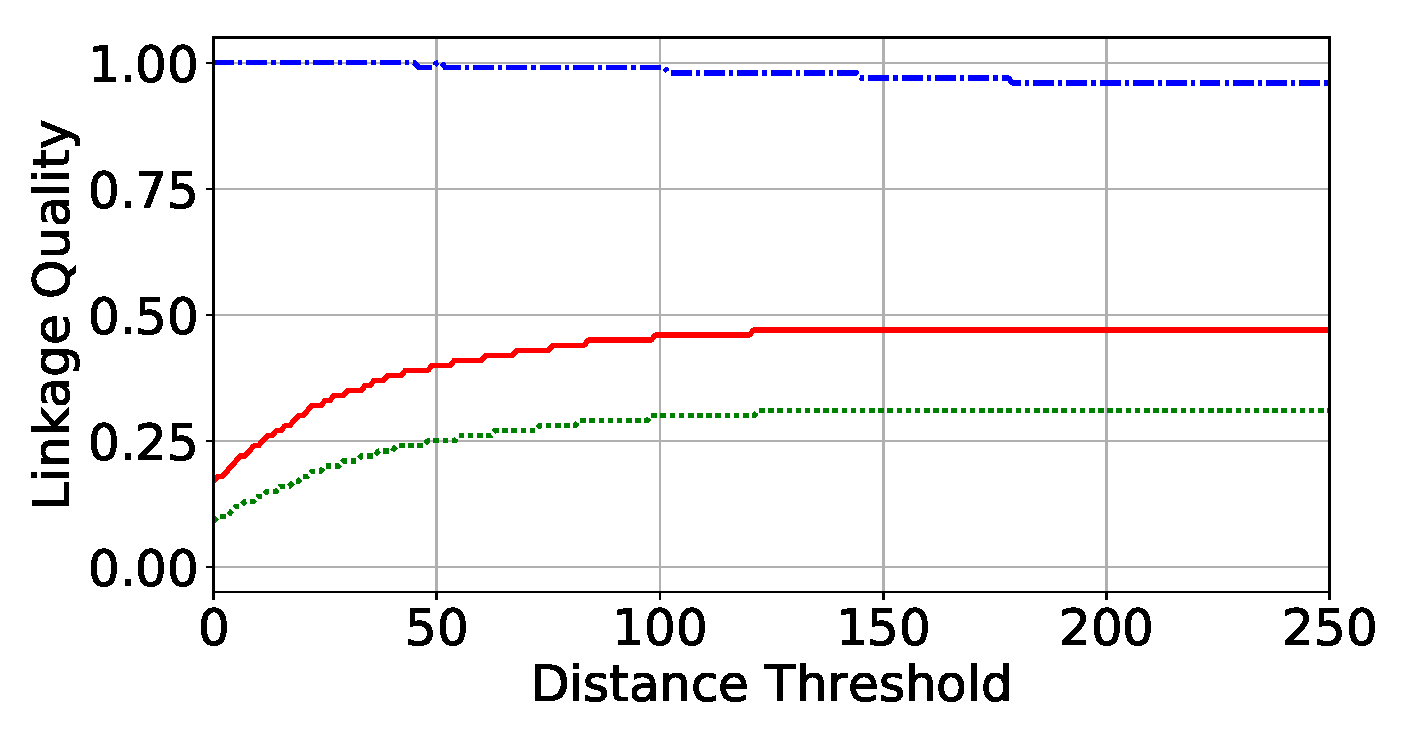
\includegraphics[width=\textwidth]{figures/plotLQ-cora-lsh-10-10}
\vspace{-6mm}
\caption{LSH using 10 bands of size 10}
\end{subfigure}
\caption{Linkage results on the Cora dataset.}
\label{cora-quality}
\end{figure}

We perform linkage on the Cora dataset using all approaches presented in
this paper: brute force, traditional blocking, LSH and M-tree, using
several selected configurations for blocking and LSH. The distance
threshold is varied between 0 and 250~\footnote{Relatively high
Levenshtein edit distances are included since Cora contains a number of
low-similarity true matches.}. For traditional blocking, the following
attributes are used individually as blocking keys: \emph{author},
\emph{title}, \emph{venue}, \emph{location}, \emph{publisher} and
\emph{year}. We also use a combined blocking key comprising all
attributes.

Figure~\ref{cora-quality} shows the precision, recall, and
F-measure~\cite{Chr12} for various thresholds~\footnote{Noting that
recent research identifies some problematic aspects with using the
F-measure to compare record linkage procedures at different similarity
thresholds~\cite{Han18}.}. As expected, low thresholds give high
precision and low recall, and the reverse for high thresholds. Brute
force and M-tree give identical results, as expected. The best linkage
quality, with an F-measure of around 0.7, is achieved by several
linkers, including brute force, M-tree, blocking on \emph{authors},
blocking on all attributes, and two of the LSH configurations. All of
these give similar overall results, apart from blocking on
\emph{authors}, which gives much better quality at very high distance
thresholds. This is due to the incomplete nature of the approach,
avoiding comparisons of significant numbers of high-similarity
non-matches and thus avoiding these becoming false positives and keeping
precision high.

For a more detailed investigation of selected linkers, the brute force
approach is used to establish a good threshold value for the Cora
dataset. The maximum F-measure is observed at a threshold value of
$d=70$. This value is dataset-dependent; for different datasets the
maximum F-measure will occur at different thresholds. In the rest of
this section we fix the threshold value at $d=70$.

\Cref{comparison-of-results-cora} shows greater detail for selected
linkers, showing the parameters for the experiment, the number of
distance comparisons made, and the precision, recall and F-measure
achieved by each algorithm. In the \emph{Linker} column the algorithm
name is followed by its parameters: for LSH the number of the bands
followed by the band size, and for traditional blocking the attributes
used for blocking. The number of distance comparisons is reported as a
machine-independent proxy for execution cost, since code profiling
shows that distance calculations are dominant.

M-tree yields the same linkage quality as brute force, although using a
significantly lower number of comparisons. This is as expected, since
both techniques are complete. Several of the incomplete linkers give
similar quality, for example \emph{LSH-2-2}, \emph{LSH-5-2},
\emph{LSH-10-2} and \emph{Block-combined}. These, and a number of other
incomplete linkers, give better precision than the complete techniques.
This is due to high-similarity non-matches, as discussed in
Sect.~\ref{sec-approach}. Although several of the incomplete linkers
give as good quality as M-tree, and in some cases at lower cost, this
is offset by the need to select appropriate configuration parameters.
Some other linkers give very poor results.

%----------------------------------------------------------------------

\begin{table}[t]
\caption{Linkage quality on Cora dataset with distance threshold $d= 70$.}
\label{comparison-of-results-cora}
\centering
\begin{footnotesize}
\begin{tabular}{lrrrr} \hline\noalign{\smallskip}
Linker~~~~~~~~~~ & ~~~Comparisons & ~~~~~Precision & ~~~~~~~~~~~Recall & ~~~~~~F-measure \\
\noalign{\smallskip} \hline \noalign{\smallskip}
Brute Force     & 1,677,025 & 0.84 & 0.57 & 0.68 \\
\noalign{\smallskip} \hline \noalign{\smallskip}
M-tree          &   902,693 & 0.84 & 0.57 & 0.68 \\
\noalign{\smallskip} \hline \noalign{\smallskip}
LSH-2-2         &   192,199 & 0.95 & 0.47 & 0.63 \\
LSH-5-2         &   342,849 & 0.91 & 0.55 & 0.69 \\
LSH-10-2        &   513,947 & 0.88 & 0.57 & 0.69 \\
LSH-2-5         &    14,329 & 0.99 & 0.28 & 0.43 \\
LSH-5-5         &    22,057 & 0.99 & 0.36 & 0.53 \\
LSH-10-5        &    26,167 & 0.98 & 0.40 & 0.57 \\
LSH-2-10        &     4,711 &    1 & 0.15 & 0.27 \\
LSH-5-10        &     6,501 &    1 & 0.19 & 0.32 \\
LSH-10-10       &    10,627 & 0.99 & 0.27 & 0.43 \\
\noalign{\smallskip} \hline \noalign{\smallskip}
Block-year      &   115,893 & 0.99 & 0.35 & 0.51 \\
Block-authors   &    11,039 & 0.94 & 0.16 & 0.28 \\
Block-title     &    27,407 & 0.95 & 0.42 & 0.58 \\
Block-venue     &    36,647 & 0.85 & 0.29 & 0.44 \\
Block-location  & 1,009,957 & 0.83 & 0.43 & 0.57 \\
Block-publisher &   833,079 & 0.85 & 0.44 & 0.58 \\
Block-combined  & 1,214,269 & 0.84 & 0.56 & 0.67 \\
\noalign{\smallskip} \hline
\end{tabular}
\end{footnotesize}
\end{table}

%----------------------------------------------------------------------

\subsection{Demographic Dataset Results}

\begin{figure}[t]
\centering
\begin{subfigure}{.46\textwidth}
  \centering
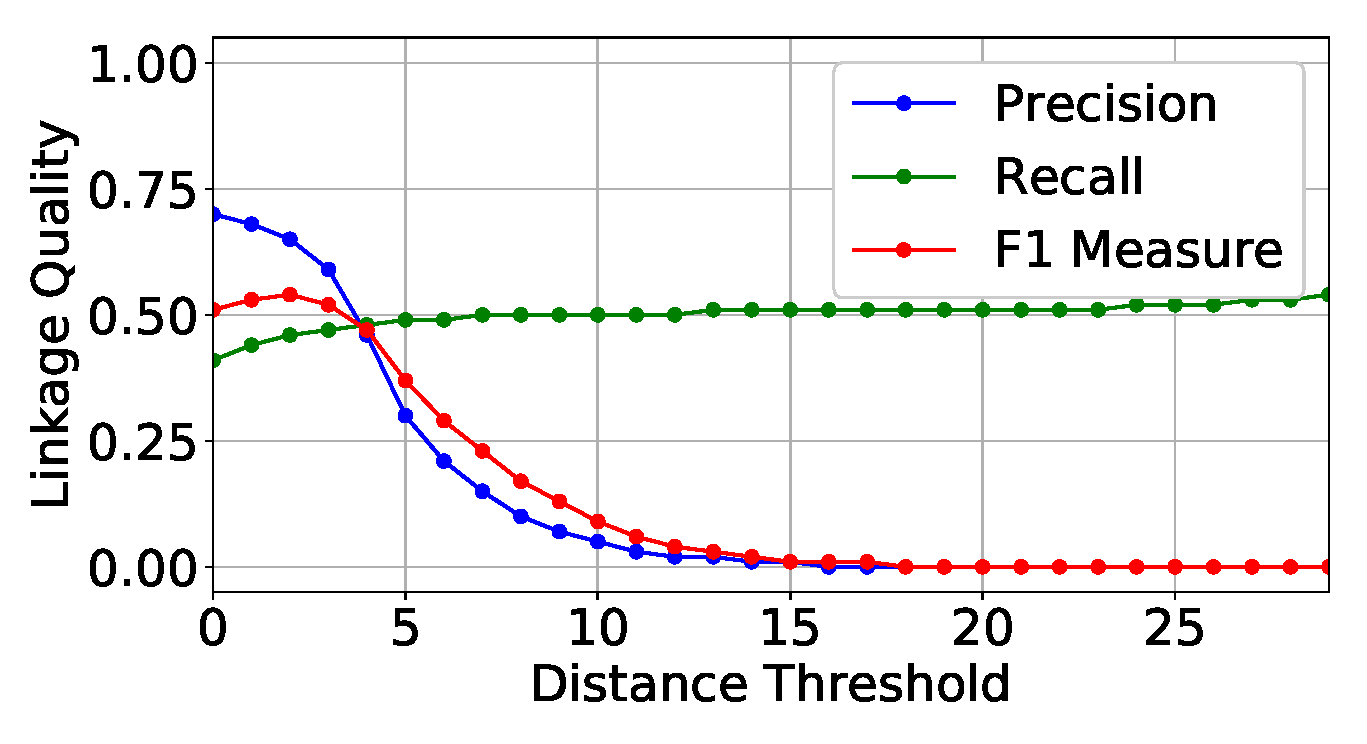
\includegraphics[width=\textwidth]{figures/plotLQ-skye-mtree}
\vspace{-6mm}
\caption{M-tree linkage on Isle of Skye \\ dataset\label{skye-quality-mtree}}
\end{subfigure}%
~~
\begin{subfigure}{.46\textwidth}
  \centering
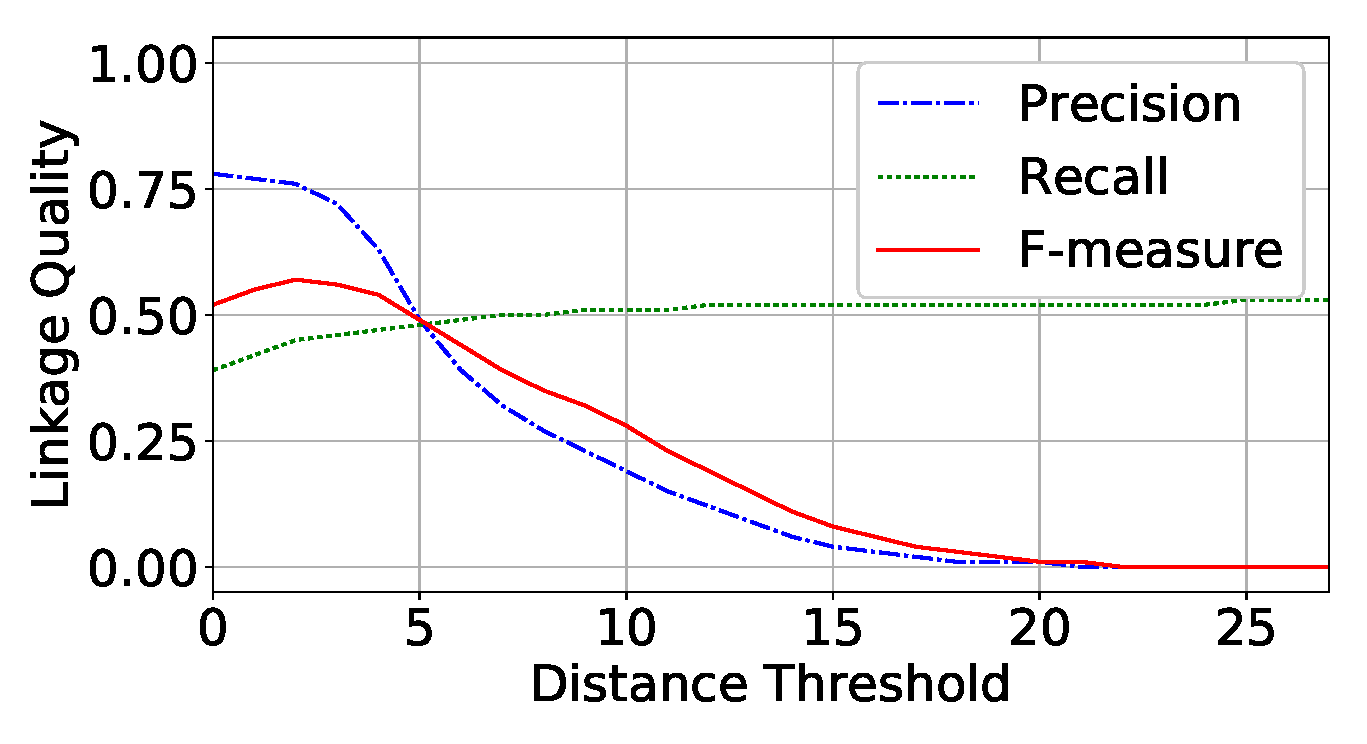
\includegraphics[width=\textwidth]{figures/plotLQ-kilmarnock-mtree}
\vspace{-6mm}
\caption{M-tree linkage on Kilmarnock \\ dataset \label{kilmarnock-quality-mtree}}
\end{subfigure} \vspace{1mm}

\begin{subfigure}{.46\textwidth}
  \centering
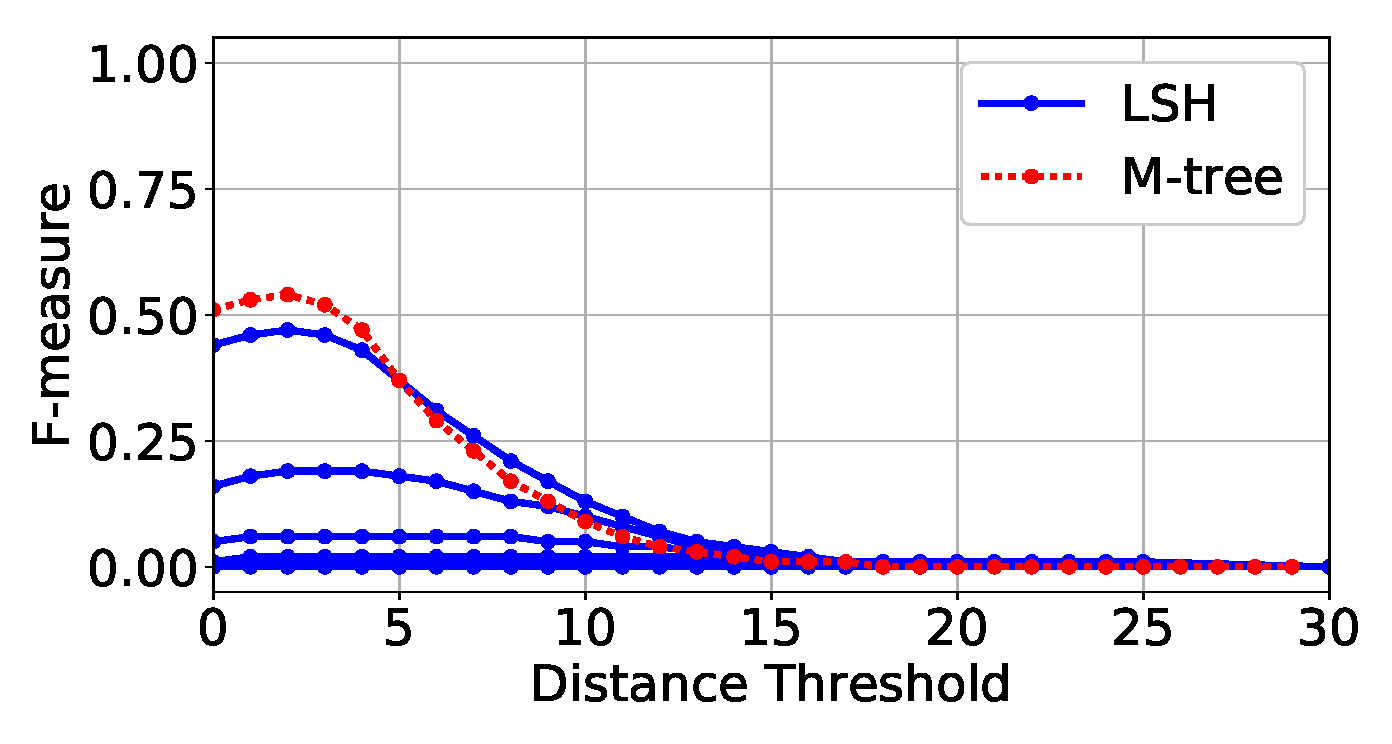
\includegraphics[width=\textwidth]{figures/plotFs-skye-f}
\vspace{-6mm}
\caption{F-measure on Isle of Skye dataset \\ with M-tree and all
LSH configurations}
\end{subfigure}%
~~
\begin{subfigure}{.46\textwidth}
  \centering
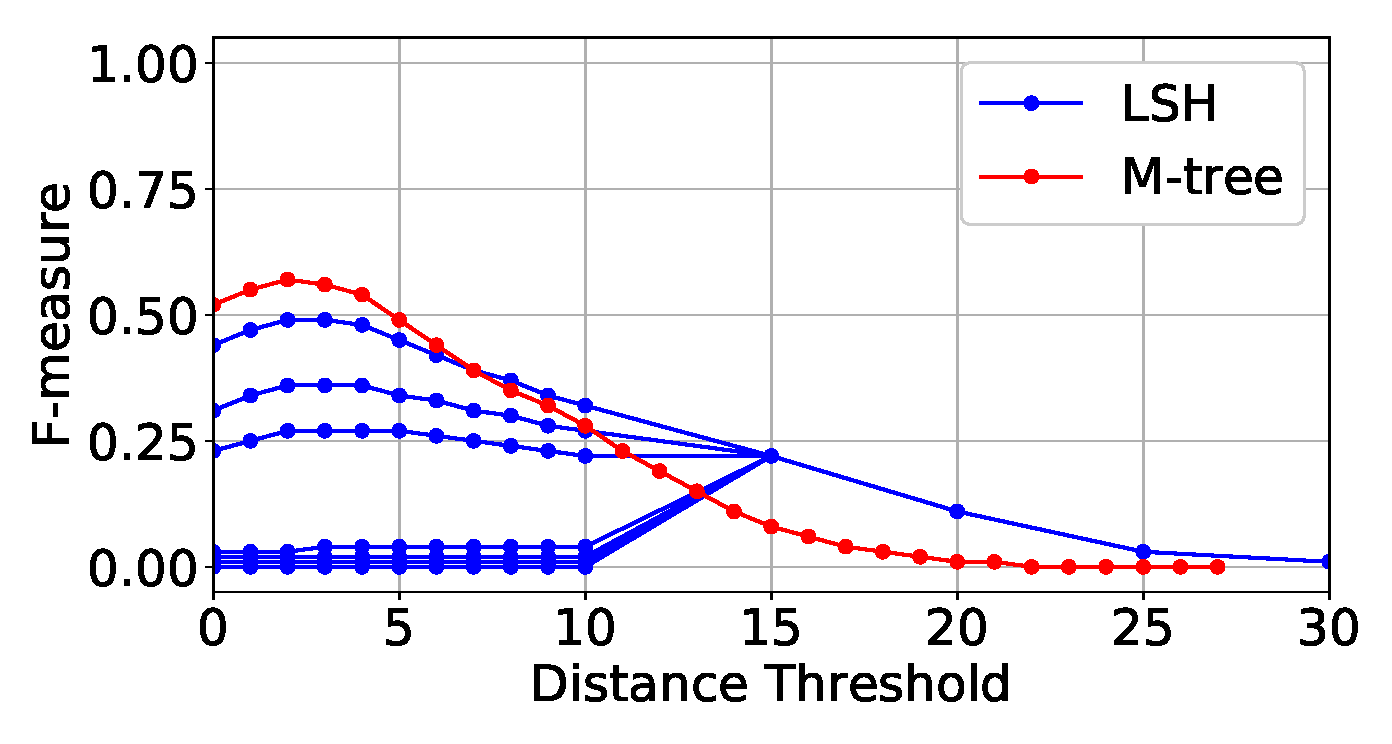
\includegraphics[width=\textwidth]{figures/plotFs-kilmarnock-f}
\vspace{-6mm}
\caption{F-measure on Kilmarnock dataset \\ with M-tree and all LSH configurations}
\end{subfigure}
\caption{Linkage results on the demographic datasets.}
\label{demography-quality}
\end{figure}

Birth records were linked to death records, separately for the Skye and
Kilmarnock datasets, using M-tree and a range of LSH configurations. It
was not computationally feasible to run the brute force linker. Of the
incomplete linkers, LSH was selected as it gave slightly better results
for Cora. The shingle size was set to $l_{ss}=2$ for all the LSH
experiments reported, as this was found to give good results and LSH
was not especially sensitive to this parameter. Results for other
shingle sizes are omitted from this paper for brevity. A lower range
of distance thresholds was explored, based on domain knowledge of the
datasets.

Figure~\ref{demography-quality} plots (a) and (b) show the M-tree precision,
recall, and F-measure for various thresholds. In both datasets, the best
F-measure values are obtained with a low distance threshold of $d=2$.
Plots (c) and (d) compare the F-measure curves for M-tree with those
obtained from a range of LSH configurations. The best F-measure value
for M-tree is higher than that of any of the LSH configurations, for
both datasets. This demonstrates both the competitiveness of M-tree
with respect to linkage quality, and its important characteristic of
being parameter-free---the linkage quality is obtained without the
need to tune for the dataset.

Tables~\ref{comparison-of-results-demography-skye}
and~\ref{comparison-of-results-demography-kili} show greater detail for
selected linkers. In both cases the F-measure achieved is better for
M-tree than any of the LSH linkers. The better linkage quality achieved
by M-tree is largely due to recall for M-tree being much higher than for
any of the LSH configurations. In most cases, LSH out-performs M-tree in
terms of precision. More significantly, LSH linkage quality is heavily
dependent on the configuration parameters. For plausible settings for
the number of bands and band size, F-measure varies from $0.01$
(extremely poor) to $0.47$ (relatively good) for Skye and from $0.03$
to $0.49$ for Kilmarnock. In both cases \emph{LSH-10-2} performs best,
but since this is data-dependent there is no guarantee that these
parameters would work well with another dataset.

The number of distance comparisons varies dramatically among the various
linkers. M-tree always performs the most comparisons, since they are
intrinsic to the \emph{range-search} algorithm. The core part of the LSH
linker performs Jaccard similarity comparisons and hashing; distance
comparisons are only performed in the final step to determine whether a
candidate pair is a link. The LSH configurations yielding the best
results perform distance comparisons of the same order of magnitude as
M-tree. This indicates that the good LSH linkers return many candidates
beyond the distance threshold. Thus, in order to get good results, LSH
tends towards a brute force search over the candidate results. Despite
this, LSH is faster due to the efficiency of the hashing process.

%----------------------------------------------------------------------

\begin{table}[t]
\caption{Linkage quality on Isle of Skye dataset with distance threshold $d=2$.}
\label{comparison-of-results-demography-skye}
\centering
\begin{footnotesize}
\begin{tabular}{lrrrr} \hline\noalign{\smallskip}
Linker~~~~~~~~~~ & ~~~Comparisons & ~~~~~Precision & ~~~~~~~~~~~Recall & ~~~~~~F-measure \\
\noalign{\smallskip} \hline \noalign{\smallskip}
M-tree   & 102,318,525 & 0.65 & 0.46 & 0.54 \\
\noalign{\smallskip} \hline \noalign{\smallskip}
LSH-2-2  &   3,109,250 & 0.63 & 0.03 & 0.06 \\
LSH-5-2  &  10,412,496 & 0.64 & 0.11 & 0.19 \\
LSH-10-2 &  53,874,127 & 0.68 & 0.36 & 0.47 \\
LSH-5-5  &      36,566 & 0.76 & 0.01 & 0.01 \\
LSH-10-5 &     129,873 & 0.72 & 0.01 & 0.02 \\
\noalign{\smallskip} \hline
\end{tabular}
\end{footnotesize}
\end{table}

%----------------------------------------------------------------------

\begin{table}[t]
\caption{Linkage quality on Kilmarnock dataset with distance threshold $d=2$.}
\label{comparison-of-results-demography-kili}
\centering
\begin{footnotesize}
\begin{tabular}{lrrrrrr} \hline\noalign{\smallskip}
Linker~~~~~~~~~~ & ~~~Comparisons & ~~~~~Precision & ~~~~~~~~~~~Recall & ~~~~~~F-measure \\
\noalign{\smallskip} \hline \noalign{\smallskip}
M-tree   & 514,871,153 & 0.76 & 0.45 & 0.57 \\
\noalign{\smallskip} \hline \noalign{\smallskip}
LSH-2-2  &  99,145,887 & 0.81 & 0.16 & 0.27 \\
LSH-5-2  & 130,721,338 & 0.79 & 0.23 & 0.36 \\
LSH-10-2 & 177,168,848 & 0.79 & 0.36 & 0.49 \\
LSH-5-5  &     239,368 & 0.84 & 0.01 & 0.02 \\
LSH-10-5 &     855,431 & 0.87 & 0.02 & 0.03 \\ 
\noalign{\smallskip} \hline
\end{tabular}
\end{footnotesize}
\end{table}

%----------------------------------------------------------------------

\section{Conclusions and Future Work\label{sec-concl}}

In this paper we have demonstrated the efficacy of MSI in achieving
complete and efficient record linkage, without the need for complex
parameter tuning. In conclusion, this claim deserves some careful
unpacking. It is always possible to achieve high quality linkage using a
brute force approach. However the quadratic complexity of this approach
prevents its practical application for datasets of even moderate size.
We have shown that MSI techniques such as M-tree can deliver high
precision, high recall results that are the same as those delivered by
brute force. Furthermore this is achieved with fewer distance
comparisons, and consistently without the need for complex parameter
tuning.

We contrast this to traditional blocking and LSH-based approaches. Their
major drawback is that whilst they can produce extremely good results,
they can also produce extremely poor results. It was our observations of
low recall given by these approaches that originally led us to
experiment with M-trees.

We note that the good results obtained by both traditional blocking and
LSH are partly due to the fact that (in the limit) they tend towards
brute force as the number of records in the blocks increase. A second,
unexpected, result is that illustrated in
Table~\ref{comparison-of-results-cora}, namely that incomplete approaches
such as LSH can in some cases yield higher precision than that achieved
by a complete method such as M-tree. This is due to the incomplete
linker masking the inability of a classifier based solely on record
similarity to correctly classify high-similarity non-matches or
low-similarity matches.

We have focused on a single distance function: the sum of
attribute-level Levenshtein distances. This gives a straightforward
intuition of record-level distances, but it is more common to normalise
metrics to the range 0-1.

Many distance functions, such as Jaro-Winkler, are not metric, and
therefore cannot be used with MSI techniques. Care must be taken to
preserve metric properties when combining metrics over individual
fields, as is highlighted in~\cite{Yujian2007}, since this may yield a
function that is not metric. It is then possible for MSI techniques to
yield results that are subtly incorrect.

Different metrics can give different distributions of inter-record
distances, which can affect both the linkage results and the number of
comparisons made, and hence the efficiency of the algorithm. Datasets
with low variation in inter-record distances are said to have high
\textit{intrinsic dimensionality}, and tend to require high numbers of
comparisons. The Scottish vital event datasets~\cite{reid2002}, combined
with Levenshtein-based metrics, appear to have high intrinsic
dimensionality. We are now, therefore, investigating the application of
various different metrics to this domain, including Jensen-Shannon,
Cosine and Structured Entropic Distance, as described
in~\cite{Connor2016}. We are also investigating the applicability of a
novel technique for dimensionality reduction~\cite{Connor2017}.

%----------------------------------------------------------------------

\section{Acknowledgements}

This work was supported by ESRC grants ES/K00574X/2 ``Digitising Scotland''
and ES/L007487/1 ``Administrative Data Research Centre---Scotland''.

We thank Alice Reid of the University of Cambridge and her colleagues,
especially Ros Davies and Eilidh Garrett, for the work undertaken on the
Kilmarnock and Isle of Skye databases.

%----------------------------------------------------------------------

\bibliographystyle{splncs03}
\bibliography{paper.bib} 

%----------------------------------------------------------------------

\end{document}

%----------------------------------------------------------------------
